% This section should include a brief presentation of the main objectives driving the formal modeling activity,
% as well as a description of the model itself, what can be proved with it, and why what is proved is important
% given the problem at hand. To show the soundness and correctness of the model, this section can show some worlds
% obtained by running it, and/or the results of the checks performed on meaningful assertions.
\subsection{Alloy Introduction}

In this section is presented the Alloy representation of some critical aspects the system must present.
It is worth highlighting that below only stable states are considered, in which the system may be found.
As a consequence, no edge cases are treated. \\
In particular, the following features are modeled:
\begin{itemize}
    \item There can't be more customers in a section than the maximum capacity of that section at any given moment.
    \item A booking is possible only by a registered customer.
    \item Every visit to the store is granted by an access title.
\end{itemize}
The super user is ignored while creating Alloy models, since they are not an integral part of the system.

\subsection{Alloy code}


\begin{lstlisting}
    //Signatures--------------------------------------

    sig Store {
        sections : some Section
    }

    sig Section {
        maxCapacity: one Int
    }{
        maxCapacity > 0
    }

    sig Email {}


    abstract sig User {
        email : one Email
    }

    sig Customer extends User {}

    some sig Manager extends User {
        store : one Store
    }

    some sig Clerk extends User {
        manager : one Manager,
        store : one Store
    }{
        manager.store = store
    }

    abstract sig AccessTitle{
        customer : lone Customer,
        sections: some Section,
        estimatedEnterTime : one Time,
        estimatedExitTime: one Time,
    }{
        estimatedEnterTime.timestamp < estimatedExitTime.timestamp
    }

    sig Ticket extends AccessTitle{
        lineNumber : one ActualLineNumber
    }

    sig Booking extends AccessTitle{
        lineNumber : one BookedLineNumber
    }{
        estimatedEnterTime.timestamp > lineNumber.timeSlot.start.timestamp
        estimatedEnterTime.timestamp < lineNumber.timeSlot.end.timestamp
        #customer = 1
    }

    sig Visit{
        accessTitle : one AccessTitle,
        enterTime : one Time,
        exitTime : lone Time
    }{
        enterTime.timestamp < exitTime.timestamp
    }

    //UTC standard format: number of seconds from 1970/01/01 00:00:00
    sig Time {
        timestamp : one Int
    }{
        timestamp>=0
    }

    sig TimeSlot {
        start : one Time,
        end : one Time
    }{
        start.timestamp < end.timestamp
    }

    abstract sig LineNumber {
        timeSlot : one TimeSlot,
        number : one Int
    }{
        number >= 0
    }

    sig ActualLineNumber extends LineNumber{}

    sig BookedLineNumber extends LineNumber{}

    //Facts------------------------------------------

    fact credentialInUsers {
        all mail : Email | mail in User.email
        no mail : Email, disj user1, user2 : User | mail in user1.email && mail in user2.email
    }

    fact everySectionInAStore {
        all section : Section | section in Store.sections
        no section : Section, disj store1, store2 : Store | section in store1.sections && section in store2.sections
    }

    fact everyLineNumberInAnAccessTitle {
        all ln : LineNumber | ln in (Ticket.lineNumber + Booking.lineNumber)
        no ln: LineNumber, disj t1, t2 : Ticket | ln in t1.lineNumber && ln in t2.lineNumber
        no ln: LineNumber, disj t1, t2 : Booking | ln in t1.lineNumber && ln in t2.lineNumber
        all disj ln1, ln2 :LineNumber | ln1.number = ln2.number => ln1.timeSlot != ln2.timeSlot
    }

    fact AVisitForEachAccessTitle {
        no at: AccessTitle, disj visit1, visit2 : Visit | at in visit1.accessTitle && at in visit2.accessTitle
    }

    fact bookOnlyAStore {
        all accessTitle : AccessTitle | one store : Store | accessTitle.sections in store.sections
    }

    fact consistentQueue {
        all disj at1, at2 : AccessTitle |
            ((at1<:Ticket).lineNumber.number < (at2<:Ticket).lineNumber.number && (at1<:Ticket).lineNumber.timeSlot = (at2<:Ticket).lineNumber.timeSlot) =>
                at1.estimatedEnterTime.timestamp =< at2.estimatedEnterTime.timestamp

        all disj at1, at2 : AccessTitle |
            ((at1<:Booking).lineNumber.number < (at2<:Booking).lineNumber.number && (at1<:Booking).lineNumber.timeSlot = (at2<:Booking).lineNumber.timeSlot) =>
                at1.estimatedEnterTime.timestamp =< at2.estimatedEnterTime.timestamp
    }

    fact noOverBooking {
        all  time : Time, section : Section |
            #{at : AccessTitle | at in
                {visit : Visit |
                    ((visit.enterTime.timestamp =< time.timestamp && visit.exitTime.timestamp>= time.timestamp) ||
                    (visit.enterTime.timestamp =< time.timestamp && visit.accessTitle.estimatedExitTime.timestamp>= time.timestamp) ||
                    (visit.accessTitle.estimatedEnterTime.timestamp =< time.timestamp && visit.accessTitle.estimatedExitTime.timestamp>= time.timestamp) )&&
                    section in visit.accessTitle.sections
                }.accessTitle
            } =< section.maxCapacity
    }

    fact equallyLongTimeSlots{
    all ts1, ts2 : TimeSlot | ts1.end-ts1.start = ts2.end-ts2.start
    }

    //Assertions--------------------------------------

    assert noMoreVisitsThanAccessTitle {
        #Visit =< #AccessTitle
    }
    check noMoreVisitsThanAccessTitle

    assert atLeastACustomerForHavingABooking {
        #Customer = 0 => #Booking=0
    }
    check atLeastACustomerForHavingABooking

    assert neverMoreCustomerThanMaxCapacity {
        all  time : Time, section : Section |
            #{c : Customer | c in
                {visit : Visit |
                    ((visit.enterTime.timestamp =< time.timestamp && visit.exitTime.timestamp>= time.timestamp) ||
                    (visit.enterTime.timestamp =< time.timestamp && visit.accessTitle.estimatedExitTime.timestamp>= time.timestamp) ||
                    (visit.accessTitle.estimatedEnterTime.timestamp =< time.timestamp && visit.accessTitle.estimatedExitTime.timestamp>= time.timestamp) )&&
                    section in visit.accessTitle.sections
                }.accessTitle.customer
            } =< section.maxCapacity
    }
    check neverMoreCustomerThanMaxCapacity

    //Worlds--------------------------------------------

    //Normal Condition
    pred world1{
        #Store=2
        #Section=3
        #User=5
        #Customer=3
        #AccessTitle=5
        #Visit=3
        #TimeSlot=5
    }

    //No Customers
    pred world2{
        #Customer=0
        #Ticket=1
        #TimeSlot=1
    }

    //Saturated Store
    pred world3{
        #Store=1
        #Section=1
        Section.maxCapacity=3
        #Visit=3
        no cus : Customer | cus not in AccessTitle.customer
        #TimeSlot=1
        #Time = 2
    }

    run world1 for 10
    run world2 for 10
    run world3 for 10


\end{lstlisting}

\subsection{World generation}

In the following paragraph are displayed examples of worlds generated
from the predicates featured in the Alloy implementation.

\begin{figure}[H]
    \centering
    \hspace*{-3.5cm}
    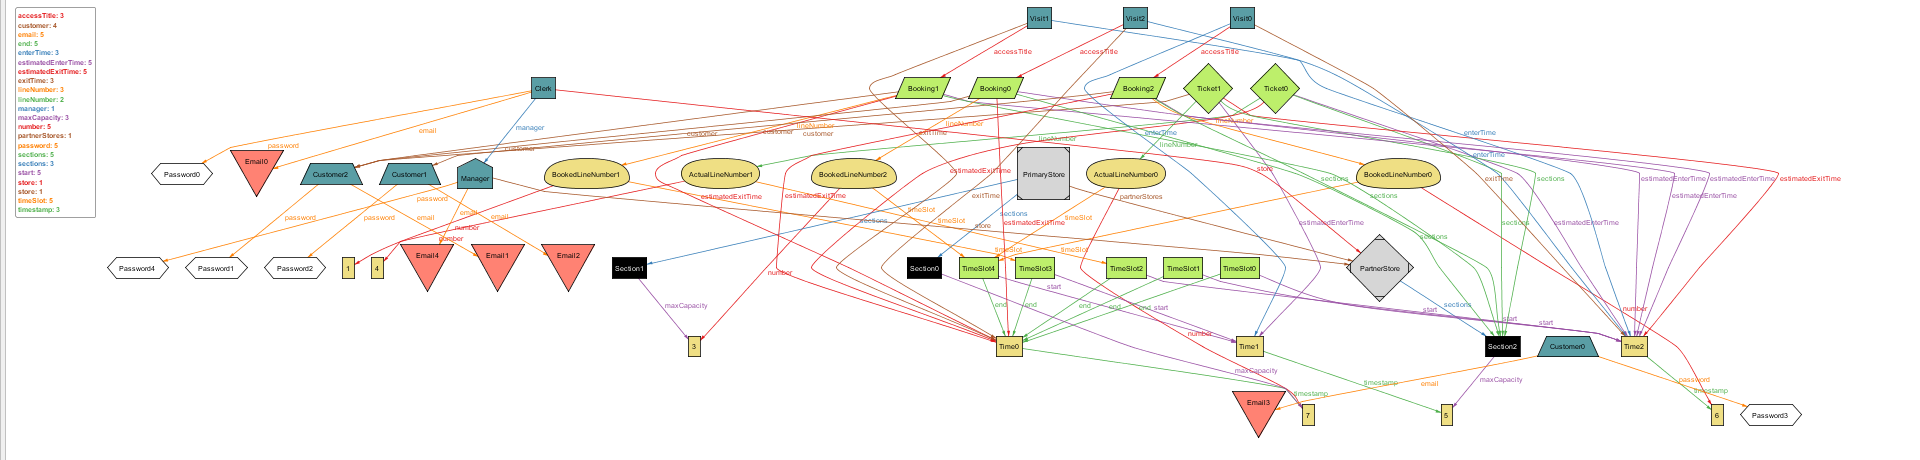
\includegraphics[height=0.7\textwidth]{Images/world1.png}
    \caption{World 1}
\end{figure}

World 1 describes the model in normal conditions, its only purpose is to show an instance of the model without checking
any particular property.

\begin{figure}[H]
    \centering
    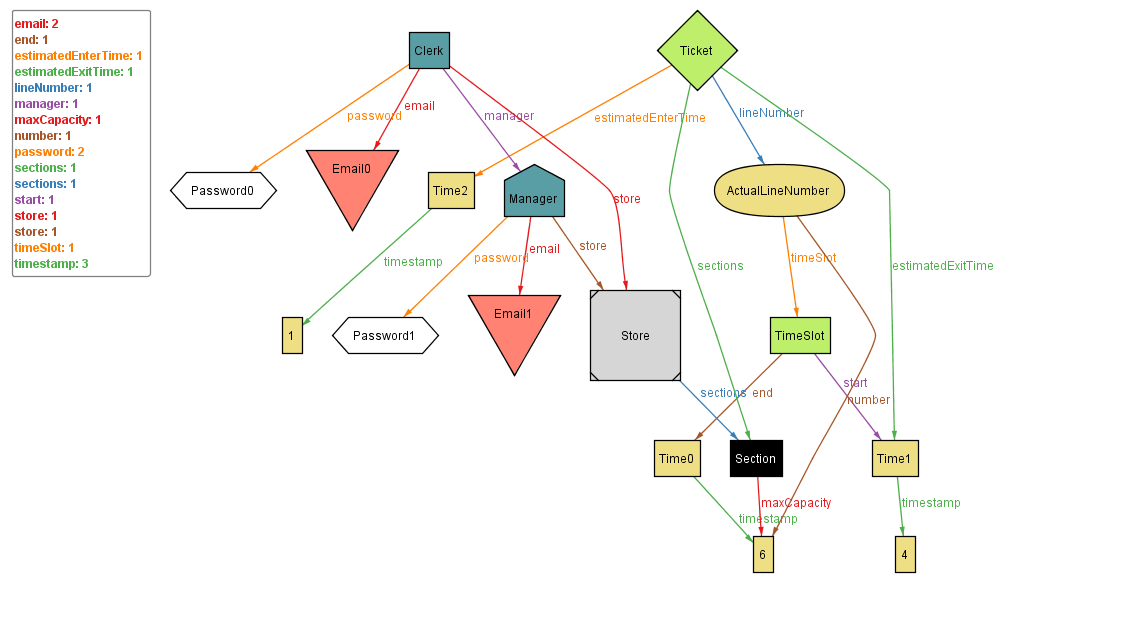
\includegraphics[height=0.5\textwidth]{Images/world2.png}
    \caption{World 2}
\end{figure}

World 2 describes the model when there are no registered customers, so that there can not be bookings and all the
tickets are made as guest going to the clerk in the store.

\begin{figure}[H]
    \centering
    \hspace*{-3.5cm}
    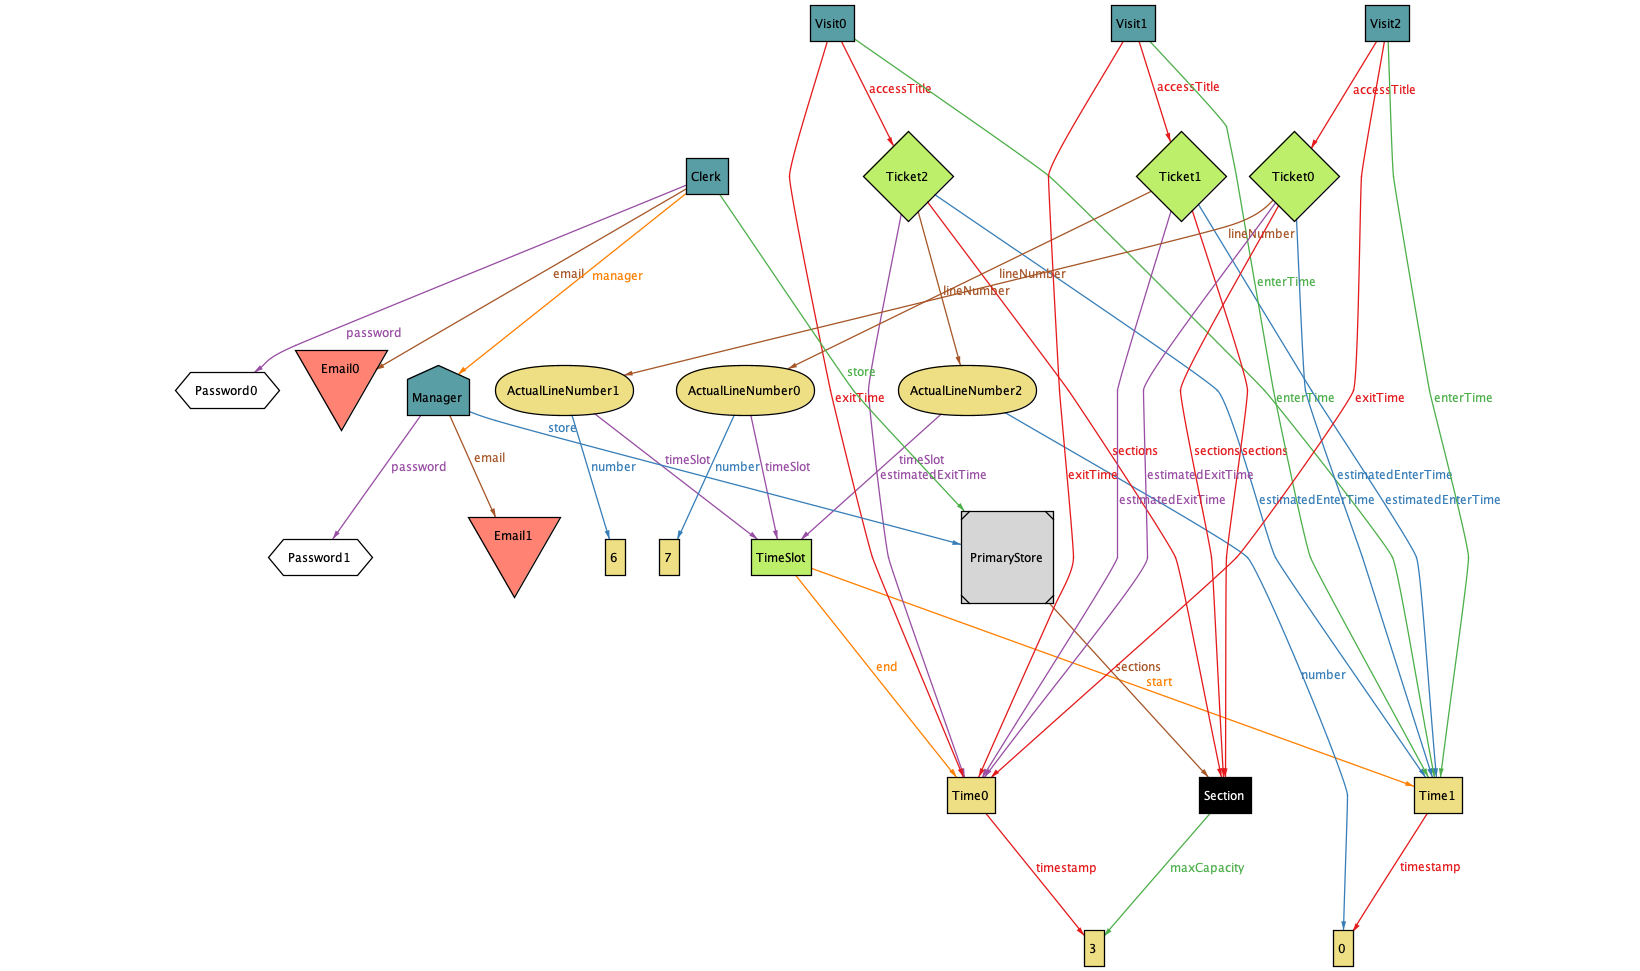
\includegraphics[height=0.7\textwidth]{Images/world3.png}
    \caption{World 3}
\end{figure}

World 3 describes the model when there is only one section and it has the same number of customers as the maximum capacity.

\subsection{Alloy Analyzer results}

6 commands were executed.\\
The results are:\\
\#1: No counterexample found. noMoreVisitsThanAccessTitle may be valid.\\
\#2: No counterexample found. atLeastACustomerForHavingABooking may be valid.\\
\#3: No counterexample found. neverMoreCustomerThanMaxCapacity may be valid.\\
\#4: Instance found.world1 is consistent.\\
\#5: Instance found.world2 is consistent.\\
\#6: Instance found.world3 is consistent.\\
